\documentclass[12pt]{article}
\usepackage[russian]{babel}
\usepackage{geometry}

%библиотеки для задания 2
\usepackage{graphicx}
\usepackage{caption}

\usepackage{enumitem}

%нестандартные математические обозначения
\usepackage{amssymb}
\usepackage{amsmath}

%различные цветовые модели
\usepackage[usenames]{color}
\usepackage[dvipsnames,table]{xcolor}
\usepackage{colortbl}

\usepackage{listings}
\usepackage{listingsutf8}
\usepackage[T2A]{fontenc}
\newcommand{\listingsttfamily}{\usefont{T2A}{PTMono-TLF}{m}{n}}

\lstset{
	language=C,                % choose the language of the code
	numbers=left,                   % where to put the line-numbers
	stepnumber=1,                   % the step between two line-numbers.        
	numbersep=5pt,                  % how far the line-numbers are from the code
	backgroundcolor=\color{black},  % choose the background color. You must add \usepackage{color}
	commentstyle=\color{Gray},
	basicstyle=\listingsttfamily\color{Gray},
	keywordstyle=\color{BurntOrange},
	stringstyle=\color{YellowGreen},
	showspaces=false,               % show spaces adding particular underscores
	showstringspaces=false,         % underline spaces within strings
	showtabs=false,                 % show tabs within strings adding particular underscores
	tabsize=4,                      % sets default tabsize to 2 spaces
	captionpos=b,                   % sets the caption-position to bottom
	breaklines=true,                % sets automatic line breaking
	breakatwhitespace=true,         % sets if automatic breaks should only happen at whitespace
	title=\lstname, 
	inputencoding=utf8,                % show the filename of files included with \lstinputlisting;
	extendedchars=\true,
	keepspaces=true
}

%параметры документа
\geometry{top=2cm, bottom=2cm, left=1cm, right=1cm}
\textheight=24cm
\textwidth=18cm
\flushbottom 

\oddsidemargin=0pt 
\topmargin=-1.5cm 
\parskip=0pt
\parindent=24pt 

\tolerance=2000 

\begin{document}
	\begin{center}
		{\parskip=1cm
			МИНИСТЕРСТВО НАУКИ И ВЫСШЕГО ОБРАЗОВАНИЯ РОССИЙСКОЙ ФЕДЕРАЦИИ
			
			ФЕДЕРАЛЬНОЕ ГОСУДАРСТВЕННОЕ БЮДЖЕТНОЕ ОБРАЗОВАТЕЛЬНОЕ УЧРЕЖДЕНИЕ ВЫСШЕГО ОБРАЗОВАНИЯ
			
			{\bf«БЕЛГОРОДСКИЙ ГОСУДАРСТВЕННЫЙ ТЕХНОЛОГИЧЕСКИЙ УНИВЕРСИТЕТ им. В. Г. Шухова»\\(БГТУ им. В. Г. Шухова)}
			
			
			\begin{figure}[bh]
			\noindent\centering{
				
\includegraphics[width=100mm]{images/start_logo.png}
				\captionsetup{labelformat=empty}
			}
			\end{figure}
			Кафедра программного обеспечения вычислительной техники и автоматизированных систем
		}
		{\parskip=0.25cm
			{\Large 
				{\bf Лабораторная работа №7}
			
				по дисциплине: <<Алгоритмы и структуры данных>>
			
				по теме: {\bf <<Структуры данных типа <<дерево>> (С)>>}
			}
		}
	\end{center}
	\begin{flushright}
		{\parskip=3cm Выполнил/a: ст. группы ПВ-231}
		
		Чупахина София Александровна
		
		Проверил:
		
		Акиньшин Даниил Иванович
	\end{flushright}
	\begin{center}
		{\parskip=3cm Белгород, 2024}
	\end{center}
	\newpage
	
	{\bf Цель работы:} изучить СД типа <<дерево>>, научиться их программно реализовывать и использовать.
	
	{\bf Задания:}
	
	\setlist[3]{noitemsep} % sets the itemsep and parsep for all level two lists to 0
	
	\begin{enumerate}
	
	\item Для СД типа <<дерево>> определить:
	
		\begin{enumerate}
	
			\item Абстрактный уровень представления СД:
			
			\begin{enumerate}
	
				\item Характер организованности и изменчивости, 
	
				\item Набор допустимых операций.
			
			\end{enumerate}
	
			\item Физический уровень представления СД:
			
			\begin{enumerate}
	
				\item Схему хранения;
	
				\item Объем памяти, занимаемый экземпляром СД;
	
				\item Формат внутреннего представления СД и способ его  интерпретации;
				
				\item Характеристику допустимых значений;
				
				\item Тип доступа к элементам.
				
			\end{enumerate}
			
			\item Логический уровень представления СД. Способ описания СД и экземпляра СД на языке программирования.
	
		\end{enumerate}
	
	\item Реализовать СД типа <<дерево>> в соответствии с вариантом индивидуального задания в виде модуля;
	
	\item Разработать программу для решения задачи в соответствии с вариантом индивидуального задания с использованием модуля, полученного в результате выполнения пункта 2 задания.
	
	\end{enumerate}
	
	\setcounter{secnumdepth}{-1} 
	\tableofcontents
	\newpage
	
	{\parskip=0.15cm
	
	\section{Задание 1:}
	\label{task_1}
	
	\subsection{Абстрактный уровень:}
	\label{task_1_1}
	\subsubsection{Задание 1.1.1:}
	\label{task_1_1_1}
	
	СД типа <<дерево>> --- нелинейная структура, в отличие от остальных СД, реализованных в лабораторных работах ранее. Дерево относится к иерархическим структурам; оно состоит из множества элементов (для дерева они называются вершинами), для которых выполняется следующее условие. В дереве обязательно есть одна начальная вершина, которая называется корнем дерева. Остальные вершины разбиты на несколько попарно непересекающихся множеств, каждое из которых тоже является деревом (поддеревом для исходного). Таким образом, формируется иерархическая связь: у корня дерева есть несколько элементов, зависящих от него, которые называются его потомками --- это как раз и будут корни поддеревьев. Но и у каждого из них есть свои несколько потомков --- корней соответствующих поддеревьев. Для каждого поддерева цепочка будет длиться, пока в множестве вершин, образующих некоторое поддерево, не останется только один элемент --- он будет корнем последнего поддерева без потомков. Такие вершины называются листьями. Количество потомков у вершины называется степенью данной вершины: максимальная степень вершины среди всех вершин дерева называется степенью дерева. Деревья со степенью $m$ = 2 называются бинарными деревьями, и в дальнейшем в этой работе, говоря о деревьях, мы будем рассматривать только их.
	
	<<Дерево>> является динамической СД: в ней могут меняться как сами элементы, так и их количество. Однако если дерево характеризуется еще каким-либо свойством (сбалансированностью, является пирамидой и т. д.), следует проводить добавление и удаление элементов так, чтобы сохранялось этой свойство. 
	
	\subsubsection{Задание 1.1.2:}
	\label{task_1_1_2}
	Для СД типа <<дерево>> определены следующие базовые операции, которые должны присутствовать в любой реализации этой структуры:
	
	\begin{enumerate}
	\item Инициализация,
	\item Создание корня,
	\item Запись данных,
	\item Чтение данных,
	\item Проверка — есть ли левый сын,
	\item Проверка — есть ли правый сын,
	\item Переход к левому сыну
	\item Переход к правому сыну
	\item Проверка — пустое ли дерево
	\item Удаление листа
	\end{enumerate}
	
	\subsection{Физический уровень:}
	\label{task_1_2}
	\subsubsection{Задание 1.2.1:}
	\label{task_1_2_1}
	Поскольку СД типа <<дерево>> является не последовательной, а иерархической, то для нее может использоваться только связная схема хранения. В дереве один элемент-родитель относится к нескольким и элементам-потомкам, и адекватно отобразить эти отношения между элементами может лишь связная схема. Таким образом, значение каждой вершины должно быть включено в структуру типа <<запись>>, которая хранит, помимо этого значения, указатели на записи, где хранятся значения вершин-потомков заданной вершины. Количество указателей зависит от степени дерева --- для бинарных деревьев оно равно двум. Если вершина является листом, все указатели на вершины-потомки должны быть пустыми; если же вершина имеет меньшее количество потомков, чем значение степени дерева, то только часть указателей являются пустыми.
	
	\subsubsection{Задание 1.2.2:}
	\label{task_1_2_2}
	Количество памяти, занимаемой СД типа <<дерево>>, зависит от того, какое количество памяти занимает его базовый тип, какое максимальное количество потомков может иметь вершина --- соответственно, сколько указателей должна содержать запись, и сколько вершин содержит дерево. Если базовый тип занимает $T$ байт, для каждого элемента необходимо также хранить 2 (поскольку здесь и далее мы рассматриваем бинарное дерево) указателей типа {\it unsigned long}, занимающего 8 байт, а дерево содержит $K$ вершин, то количество памяти, занимаемой экземпляром СД <<дерево>>, будет равно $(T+2)*K$ байт.
	
	\subsubsection{Задание 1.2.3:}
	\label{task_1_2_3}
	Найти количество 
	Так как СД типа <<дерево>> с количеством вершин K использует связную схему хранения, то значения записей, представляющих отдельные вершины дерева, могут храниться в памяти независимо друг от друга. В некоторых реализациях дерево может представляться массивом, где хранятся записи, отображающие вершины, но и в этом массиве они не обязательно идут подряд. Значения в полях записей также могут храниться в памяти компьютера не подряд (либо в порядке, отличном от заданного). Значение элемента переводится в двоичный код в зависимости от базового типа; указатели кодируются как положительные целые числа --- переводятся в двоичную систему счисления и дополняются нулями слева до размера в 8 байт.

	\subsubsection{Задание 1.2.4:}
	\label{task_1_2_4}
	
	Найти количество допустимых значений для СД типа <<бинарное дерево>> сложнее, чем для рассматриваемых ранее структур: ведь помимо допустимых значений самих вершин и их количества в дереве, необходимо учесть и их порядок, а он гораздо сложнее, чем таковой у линейных структур. Впрочем, для фиксированного набора значений для $i$ вершин существует формула, показывающая, сколько различных бинарных деревьев можно составить из такого набора: их количество будет равно $\frac{(2i)!}{(i + 1)(i!)^2}$. Соответственно, просуммировав все значения этого выражения по $i$ от 1 до некоторого $max$ (максимальное количество элементов определяется объемом памяти, отведенным для хранения дерева), получим, сколько различных конфигураций бинарных деревьев существует вообще: $$\sum_{i = 1}^{max}{\frac{(2i)!}{(i + 1)(i!)^2}}$$ Кардинальное число для СД типа <<бинарное дерево>> c базовым типом BaseType в итоге находится как: $$(\sum_{i = 1}^{max}{\frac{(2i)!}{(i + 1)(i!)^2}} \times CAR(BaseType)) + 1$$.
	
	\subsubsection{Задание 1.2.5:}
	\label{task_1_2_5}
	СД типа <<дерево>> имеет последовательный доступ к элементам: поиск нужного элемента для чтения или записи осуществляется с помощью перехода к левому или правому сыну текущего элемента. 
	
	\subsection{Логический уровень:}
	\label{task_1_3}
	СД типа <<дерево>> является производной СД, и потому сначала необходимо реализовать ее тем или иным способом. Только после этого ее можно описать на логическом уровне (представить на языке программирования). Приведем здесь описания для той реализации, которая будет выполнена в задании 2 этой лабораторной работы (дерево в динамической памяти с базовым типом <<целое число>>).
	
	\lstinputlisting{../АСД 7 си/example.c} 
	
	Заполнение экземпляра СД типа <<дерево>> значениями и добавление в него новых элементов без модуля с функциями для работы с этой СД весьма трудоемко, а потому не будем его демонстрировать. Займемся написанием этого модуля в задании 2.
	
	\begin{center}
	{\bf Индивидуальное задание; вариант 21}
	\end{center}
	{\bf Модуль 1:} Дерево в динамической памяти (базовый тип определяется задачей).
	
	{\bf Реализация на языке C:}
	
	{\it \#if !defined(\_\_TREE1\_H)
		
		const TreeOk = 0;
		
		const TreeNotMem = 1;
		
		const TreeUnder = 2;
		
		typedef	/*определить !!!*/ BaseType;
		
		typedef struct element *ptrel;
		
		typedef struct element\{basetype data;
			
			ptrel LSon;
			
			ptrel RSon;
		\}
			
		typedef PtrEl *Tree;
		
		short TreeError;
		
		void InitTree(Tree *T)// инициализация — создается  элемент, который будет содержать корень дерева
		
		void CreateRoot(Tree *T) //создание корня
		
		void WriteDataTree(Tree *T, BaseType E) //запись данных
		
		void ReadDataTree(Tree *T,BaseType *E)//чтение
		
		int IsLSon(Tree *T)//1 — есть левый сын, 0 — нет 
		
		int IsRSon(Tree *T)//1 — есть правый сын, 0 — нет 
		
		void MoveToLSon(Tree *T, Tree *TS)// перейти к левому сыну, где T — адрес ячейки, содержащей адрес текущей вершины, TS — адрес ячейки, содержащей адрес корня левого поддерева(левого сына)
		
		void MoveToRSon(Tree *T, Tree *TS)//перейти к правому сыну
		
		int  IsEmptyTree(Tree *T)//1 — пустое дерево,0 — не пустое
		
		void DelTree(Tree *T)//удаление листа
		
		\#endif
	}

	
	{\bf Задача 2:} 
	
	\begin{description}
		\item[а)] {\it Procedure BildTree(var T:Tree)};
		
		Строит дерево арифметического выражения, заданного в ППЗ. Операнды — целочисленные константы. Операции — «+», «–», «*» и «div».
		
		\item[б)] {\it Procedure WritePostfix(T:Tree);}
	
		Выводит арифметическое выражение в ОПЗ.
	
		\item[в)] {\it Function WriteCalc(T:Tree):integer;}
	
		Вычисляет значение по дереву арифметического выражения и выводит результат выполнения каждой операции в виде: <операнд><операция><операнд>=<значение>
	\end{description}
	
	\section{Задание 2:}
	\label{task_2}
			
	Разделим код выполнения этого задания на два файла: заголовочный и  реализации. В заголовочном файле зададим константы с кодами трех основных ошибок, которые могут возникнуть в ходе работы со списками: TreeNotMem --- не удалось выделить место под хранение нового элемента-записи ; TreeUnder --- попытка записать элемент в пустое дерево либо прочесть элемент из него. Под хранение кода ошибки отводится переменная. После этого дадим название используемым типам данных: BaseType --- тип, элементы которого хранит список (в нашем случае это целые числа int: почему был выбран именно этот тип, поясним при рассмотрении задания 3); element --- запись, состоящая из значения вершины и двух указателей на такие же записи --- на левый и правый потомки вершины; PtrEl --- указатель на экземпляр element; Tree --- указатель на экземпляр PtrEl. Немного подкорректировав данный для варианта 21 шаблон, получим такой заголовочный файл:
		
	\lstinputlisting{../АСД 7 си/tree.h} 
		
	Реализация функций будет вынесена в отдельный файл со следующим содержанием.
		
	\lstinputlisting[]{../АСД 7 си/Tree.c} 
		
	Для нормальных (не вызывающих ошибки и аварийного завершения) сценариев этих функций можно составить автоматизированные тесты и вынести их в отдельный файл тестирования. Будем тестировать функции следующим образом. Сначала рассматривая сценарии выполнения для дерева из одного элемента, а после написания тестов для функций перемещения по дереву, MoveToLSon и MoveToRSon, для некоторых функций рассмотрим также и сценарии, где дерево имеет больше одного элемента. Также везде, кроме как в тестах функций записи и чтения значений, WriteDataTree и ReadDataTree, не будем заполнять значениями созданные деревья.
		
	\lstinputlisting{../АСД 7 си/tree_test.c} 
		
	Запустив программу, можем самостоятельно убедиться, что все тесты прошли успешно:
	
	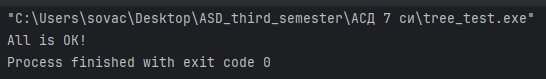
\includegraphics[width=170mm]{images/tree_test_output.png} 
	
	\section{Задание 3:}
	\label{task_3}
	
	Теперь, когда модуль для СД типа <<дерево>> реализован, можем перейти к решению задачи для варианта 21, описанной выше. Базовым типом дерева для этой задачи будет целое число. Как сказано в условии, операндами выражения должны быть целые числа; сами же операции (их всего четыре: сложение, вычитание, умножение, деление нацело) можно обозначать константами 0, 1, 2, 3 соответственно. Ведь при построении дерева арифметического выражения операнды будут его листьями, а операции --- вершинами с потомками. И определить, как стоит толковать целое значение вершины --- как число или как код операции --- очень просто: нужно лишь знать, имеет ли вершина потомков. Затем объявим два вспомогательных массива для связи целочисленных <<кодов>> операций с их обозначениями в строке (<<+>>, <<->>, <<*>>, <</>> соответственно) и функциями, которым соответствуют эти операции. В этих массивах символы, обозначающие операции, и функции идут в указанном выше порядке. 
	
	Откорректировав прототипы функций, данные в индивидуальных заданиях, для языка C, можем реализовать их следующим образом.
	
	{\bf Примечание:} при вводе с клавиатуры рассчитываем, что соблюдаются следующие правила: операнды и операции отделены друг от друга одним пробелом, унарный минус применяется только к отдельным числам и не отделяется пробелом от числа, с которым связан.
	
	\lstinputlisting{../АСД 7 си/task.c} 
	
	Для того, чтобы протестировать полученную программу, будем использовать следующие выражения: а) 3 * 6 - 25 / 4 + 1 --- выражение, для отображения которого в инфиксной записи не требуются скобки, б) (6 + 231 / 15) * (4 + 3) --- выражение, для отображения которого в инфиксной записи скобки необходимы, в) 5 * (-7 - 9 / -4) --- пример с отрицательными числами. В префиксной записи они будут выглядеть так: а) + - * 3 6 / 25 4 1; б) * + 6 / 231 15 + 4 3; в) * 5 - -7 / 9 -4. Для каждой из полученных префиксных записей запустим программу и введем ее с клавиатуры. Вывод будет следующим:
	
	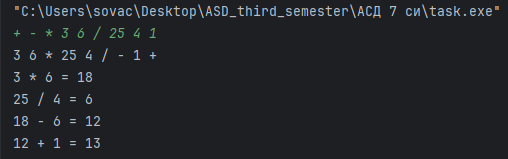
\includegraphics[width=120mm]{images/expression1.png} 
	
	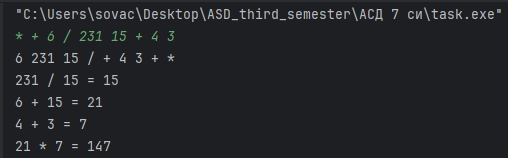
\includegraphics[width=120mm]{images/expression2.png} 
	
	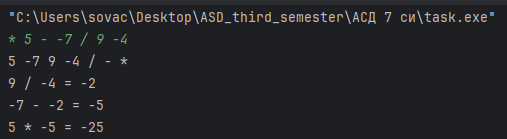
\includegraphics[width=120mm]{images/expression3.png} 
	
	Как можно убедиться, постфиксные (обратные польские) записи построены верно, значения выражений также вычислены без ошибок.
	
	\section{Вывод:}
	
	В ходе лабораторной работы дали характеристику СД типа <<дерево>>, форматам ее представления, реализовали один из них в соответствии с вариантом (дерево в динамической памяти с базовым типом <<целое число>>), написали ряд базовых функций для работы с деревьями в этом формате, а также решили задачу ввода и хранения арифметического выражения с операциями сложения, вычитания, умножения и деления нацело в формате дерева, вывода этого выражения на экран и его вычисления.
}
\end{document}